%%%%%%%%%%%%%%%%%%%%%%%%%%%%%%%%%%%%%%%%%%%%%%%%%%%%%%%%%%%%%%%%%%
\section{Quality Assurance}
\label{sec:fdsp-apa-qa}

%\subsection{Component Testing}
%\label{sec:fdsp-apa-qa-testing}

%\fixme{PSL: input needed. are there old tests of APA components we want to present here?  things like the long-term wire tension studies, etc.}  

The most important and complete information for assuring the quality of the \dword{apa} design, components, materials, and construction methods comes from the construction and operation of \dword{pdsp}.  We have already learned much about design, component testing, and fabrication procedures that is informing the detailed design and plans for the DUNE \dword{apa} construction project. \dword{pdsp} included six full-scale \dword{dune} \dwords{apa} instrumenting two drift regions around a central cathode.  Four of the \dword{pdsp} \dword{apa}s were constructed in the USA at %the University of Wisconsin 
PSL, and two were made at Daresbury Laboratory in the UK. All were shipped to \dword{cern}, integrated with photon detectors and \dword{ce} and tested in a \coldbox prior to installation into the \dword{pdsp} cryostat.  Figure~\ref{fig:sp-apa-pd-photo} shows a photo of one of the drift regions in the fully constructed ProtoDUNE detector.

\begin{dunefigure}[ProtoDUNE-SP photo]{fig:sp-apa-pd-photo}
{One of the two drift regions in the \dword{pdsp} showing the three installed \dwords{apa} on the left.}
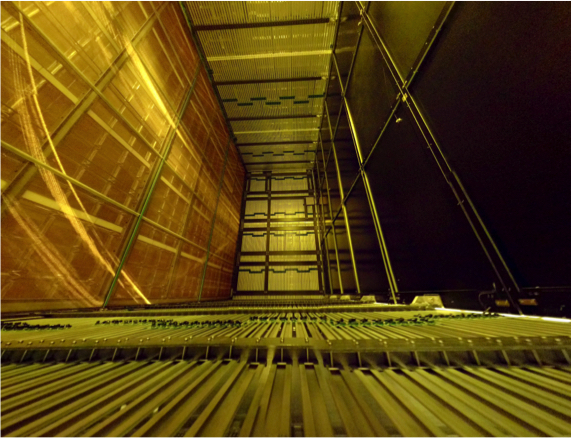
\includegraphics[width=0.7\textwidth]{sp-apa-protodune-photo.jpg}
\end{dunefigure}

\subsection{Results from ProtoDUNE-SP Construction}
\label{sec:fdsp-apa-qa-protodune-const}

A thorough set of \dword{qc} tests were performed and documented throughout the fabrication of the \dword{pdsp} \dword{apa}s.  The positive outcomes give great confidence in the quality of the overall \dword{apa} design  and construction techniques.  Here we summarize some of the testing that was done for \dword{pdsp} and the results.   

%All printed circuit boards (PCBs) were electrically tested and cleaned according to IPC standard. Dimensional checks were performed and all solder pads checked for damage. Any boards that required corrective machining were washed thoroughly, and PCBs were always handled with gloves to prevent contamination.

After each wire layer was applied to an \dword{apa}, continuity between the head and foot boards was checked.  This test is most useful for the $U$ and $V$ layers, where metal traces on the side boards can be damaged during construction. All boards were visually inspected as construction proceeded.

Also after each wire layer was finished, channels were checked for isolation.  In the beginning wire-to-wire isolation was measured. Those measurements took a lot of time and no problems ever arose.  In the end, each wire was individually hi-pot tested at \SI{1}{kV}. No failures were ever seen. However, leakage currents were seen to be highly dependent on relative humidity.  The surface of the epoxy has some affinity for moisture in the air and provides a measurable leakage path when relative humidity exceeds about \SI{60}{\%}.

Wire tension was measured for all wires at production. Wire tension measurements were performed again for a subset of wires on each \dword{apa} after arriving at \dword{cern}.  Based on the traveler documents provided by the production sites, wires having outlier tension values were selected from each \dword{apa} for re-measurement at \dword{cern}. In addition, a set of randomly selected wires from each plane were measured. In total, for six \dword{apa}s, $\sim$1500 wires had their tension re-measured at \dword{cern}. Measurements took place in the clean room with \dword{apa}s hanging vertically, the first time the tensions were sampled in this orientation. Tension measurements were performed by using the laser-photodiode based method, the same as at the production sites. Figure~\ref{fig:sp-apa-pd-tension} shows the comparison of tension values measured at \dword{cern} versus at production site for the selected subset of wires from each wire plane.

\begin{dunefigure}[ProtoDUNE-SP wire tension measurement plots]{fig:sp-apa-pd-tension}
{Comparison of wire tensions upon arrival at \dword{cern} versus at the production sites for a sample of wires on each of the \dword{pdsp} \dword{apa}s.}
\mbox{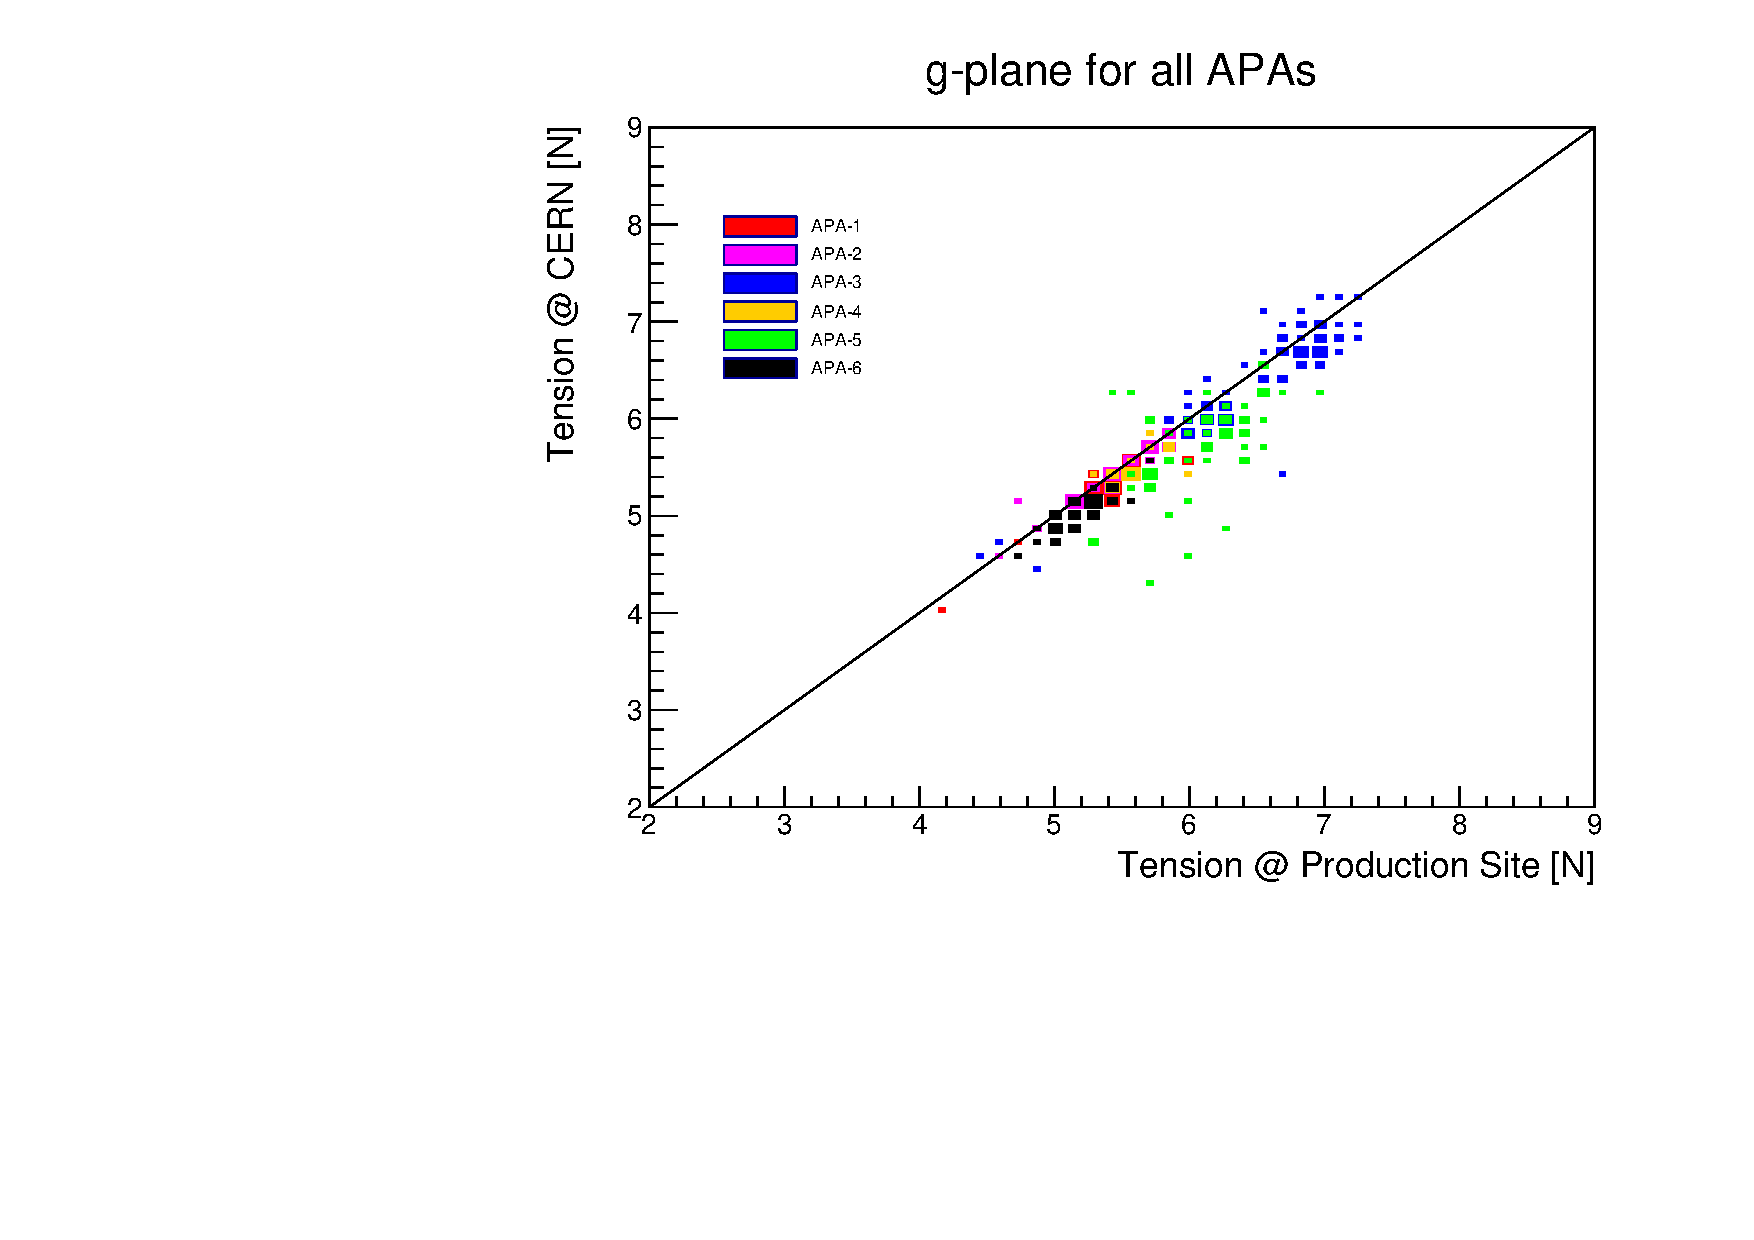
\includegraphics[height=0.23\textheight]{sp-apa-PD-tension-prod-cern-G.pdf} %\hspace{1mm}
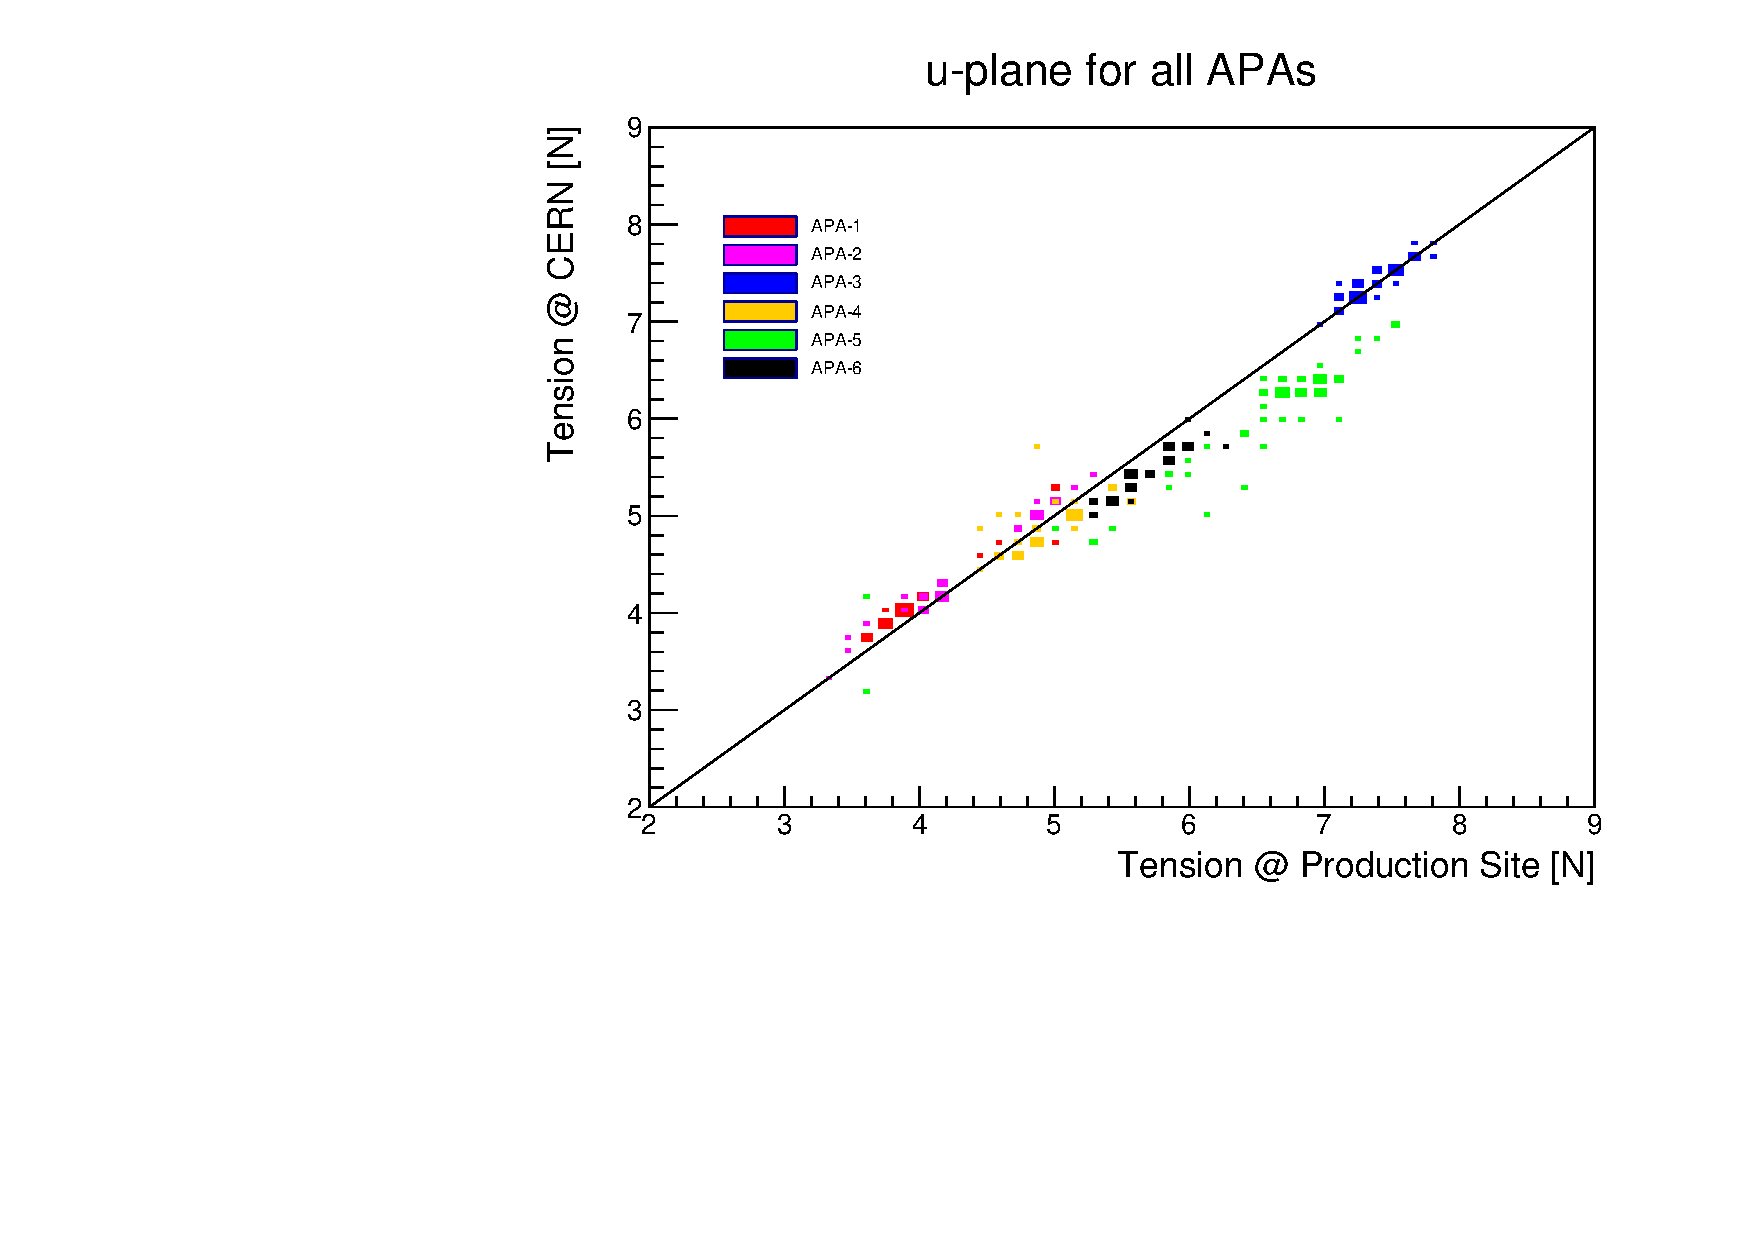
\includegraphics[height=0.23\textheight]{sp-apa-PD-tension-prod-cern-U.pdf}} \\
\vspace{3mm}
\mbox{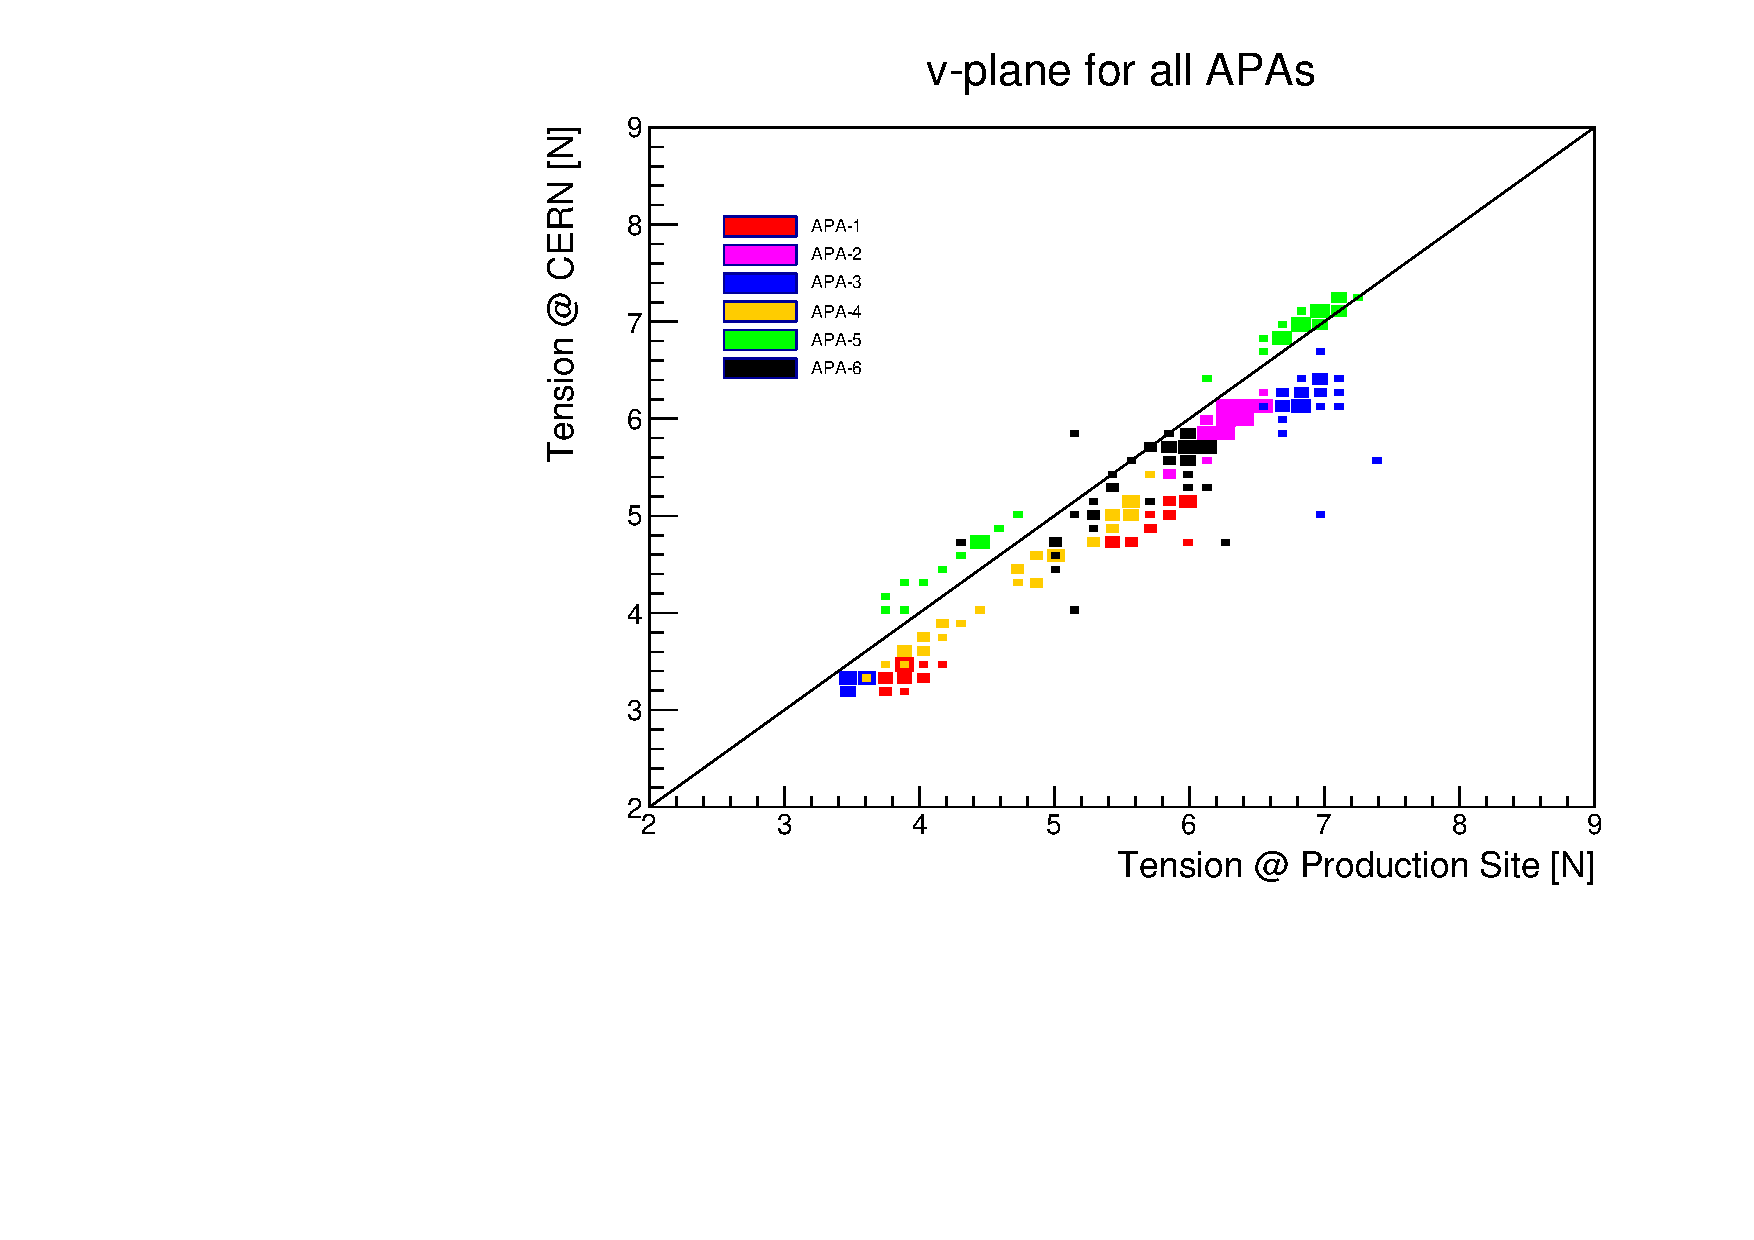
\includegraphics[height=0.23\textheight]{sp-apa-PD-tension-prod-cern-V.pdf} %\hspace{1mm}
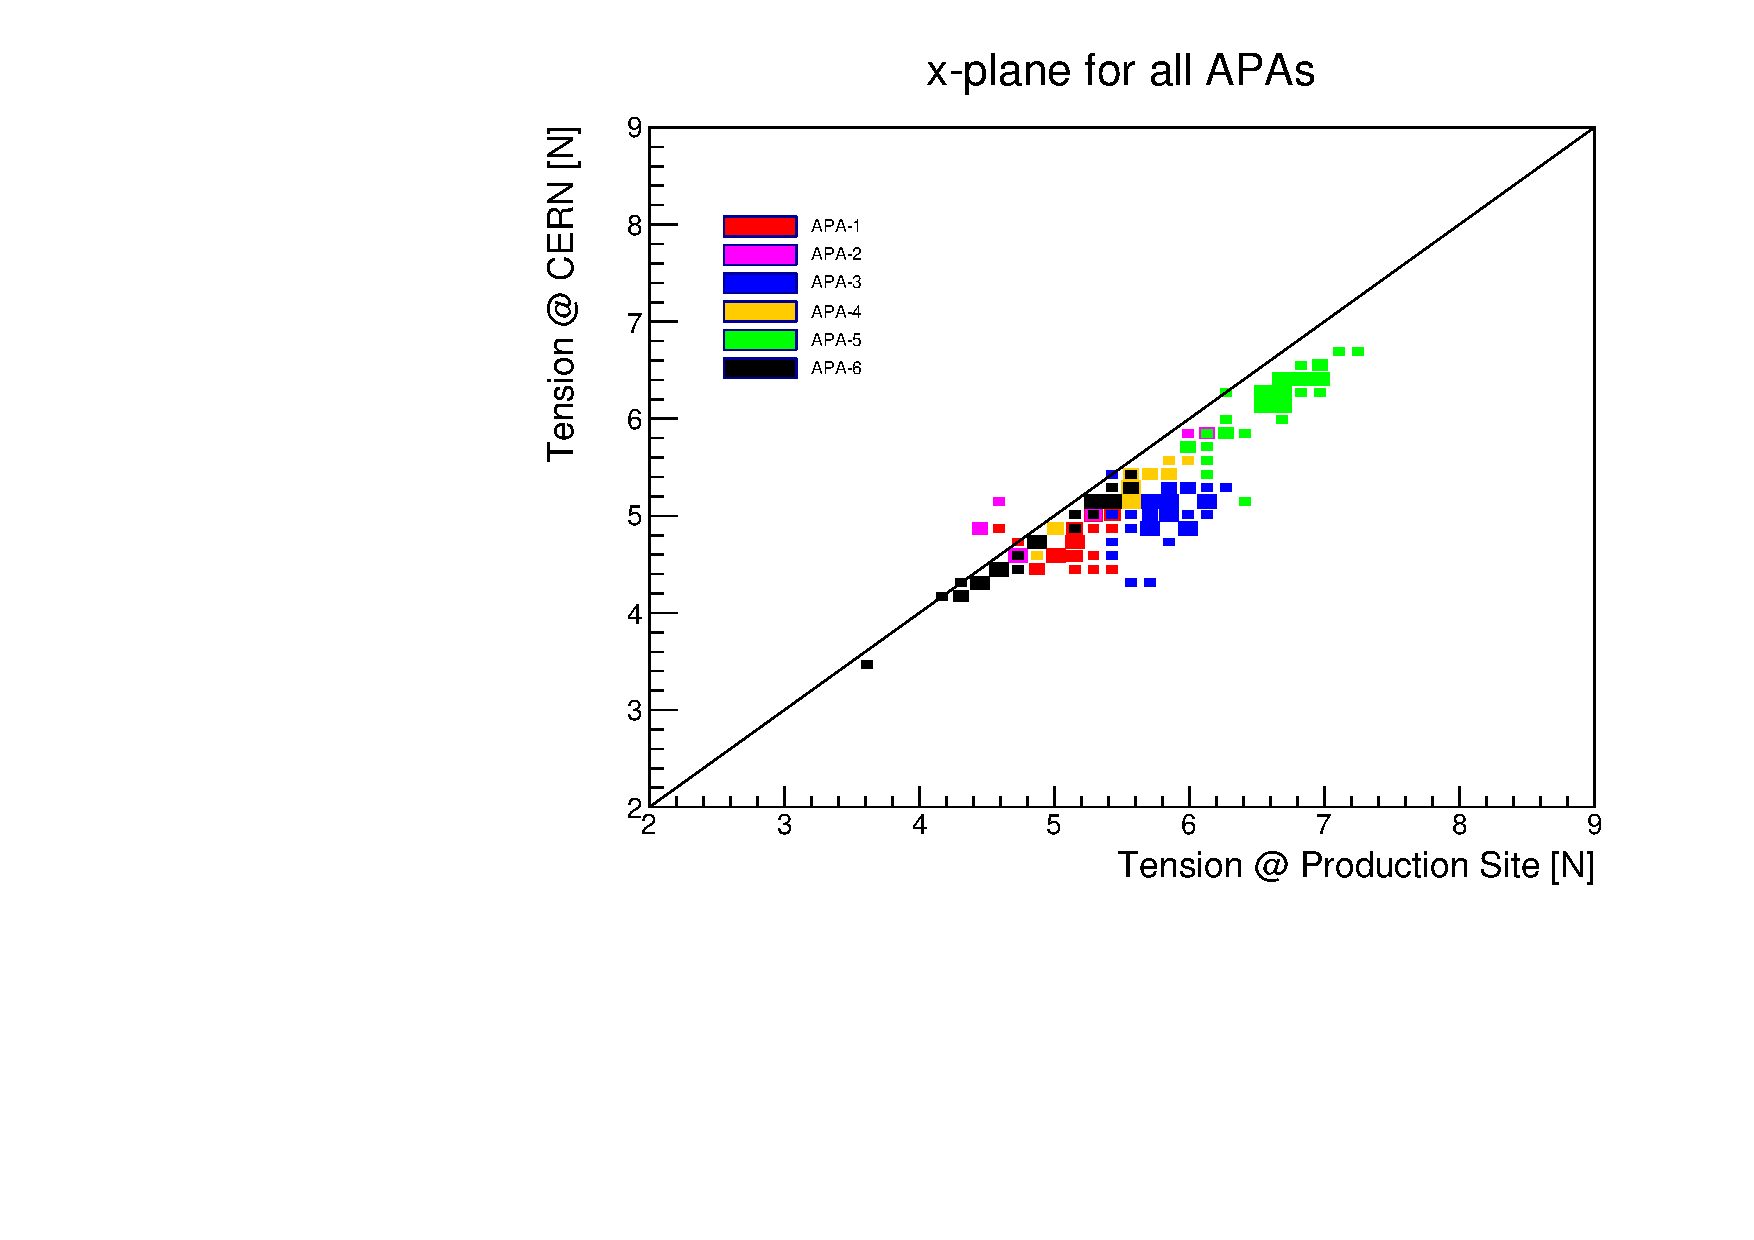
\includegraphics[height=0.23\textheight]{sp-apa-PD-tension-prod-cern-X.pdf}}
\end{dunefigure}

To test if a cold cycle had any effect on the wire tension, samples of wires had their tension measured again after the cold-box tests at \dword{cern}. This is the only tension data we have after a cold-cycle for \dword{pd} \dword{apa}s. The results are presented in Figure~\ref{fig:sp-apa-pd-tension-cold}, which shows no significant change in the resonant frequency of the wires, indicating cold cycle does not have any significant effect on wire tension.

\begin{dunefigure}[ProtoDUNE-SP wire tension before and after cold tests]{fig:sp-apa-pd-tension-cold}
{Comparison of wire tensions after the \coldbox test versus before at \dword{cern} for a sample of wires on each of the \dword{pdsp} \dword{apa}s.}
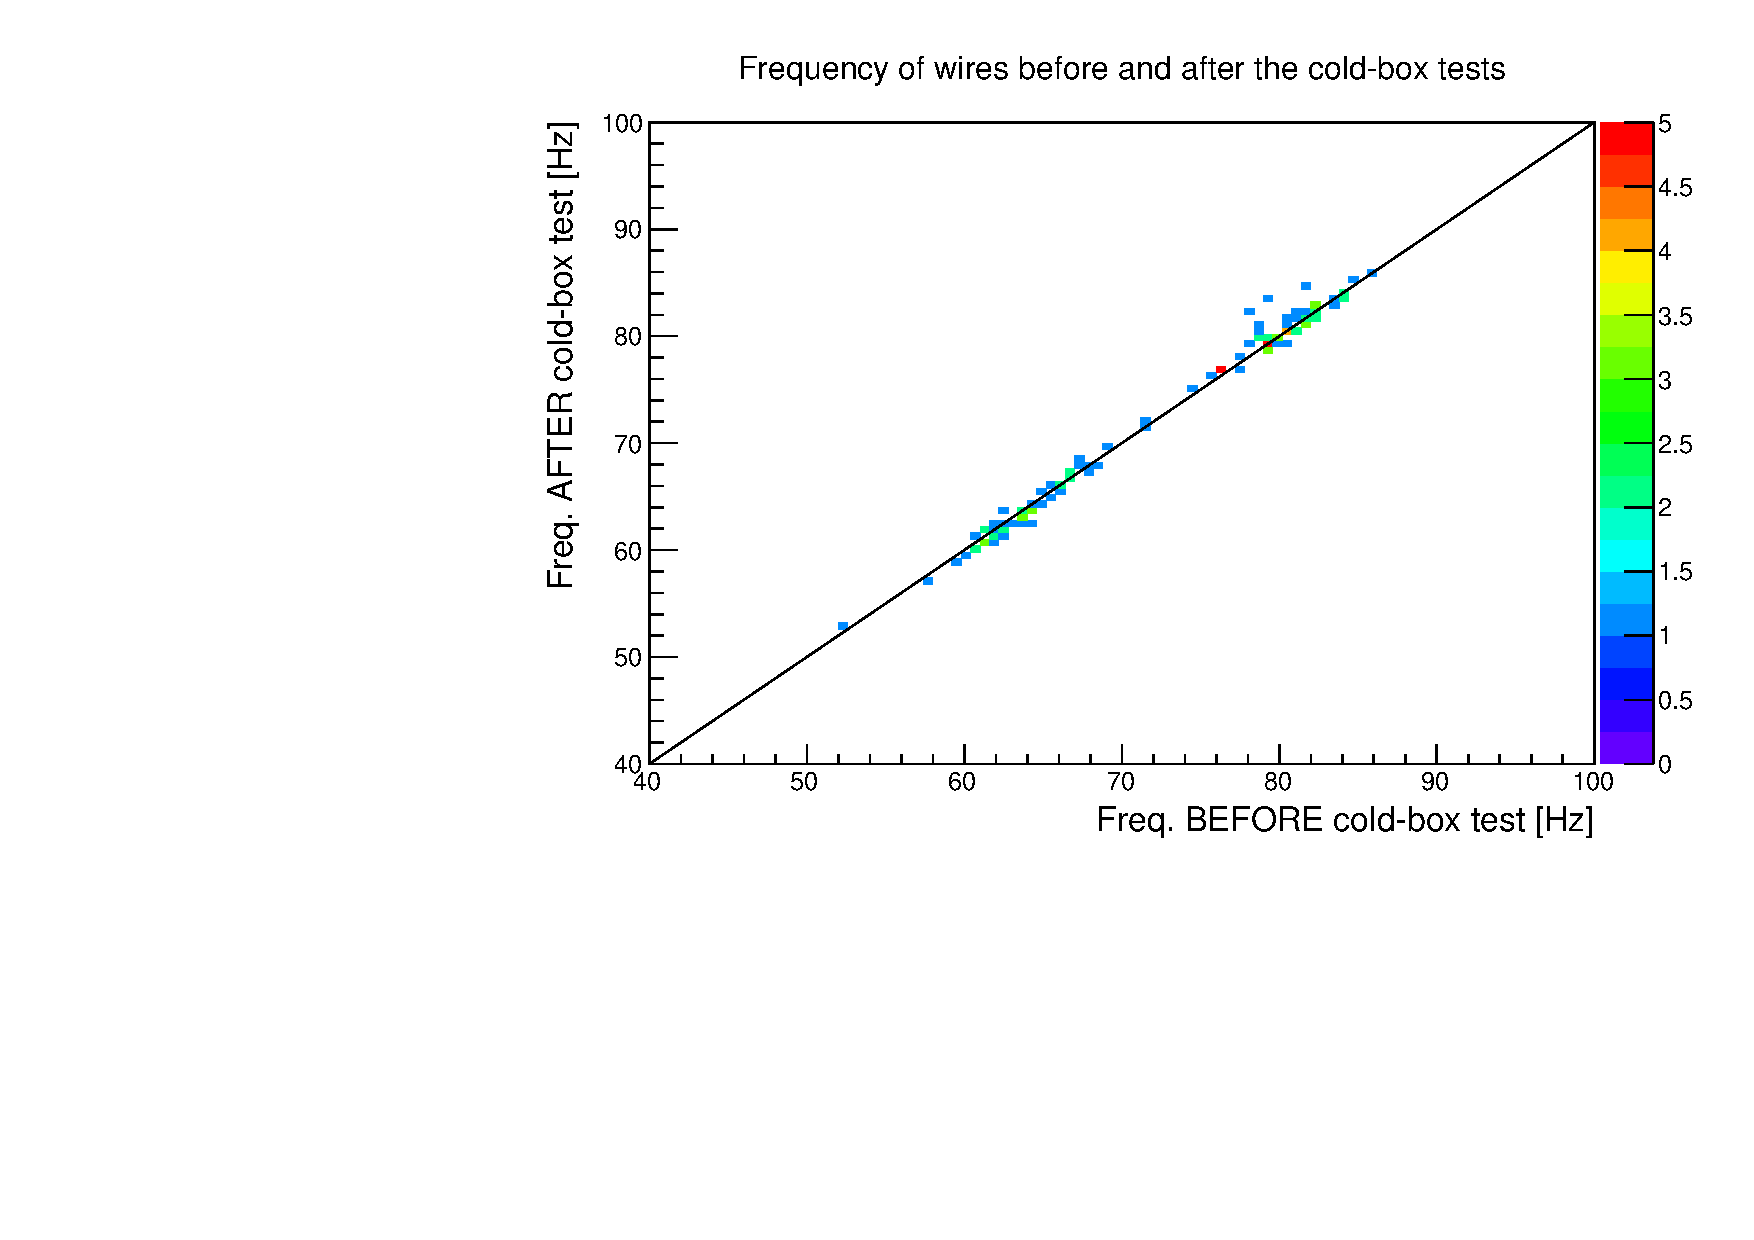
\includegraphics[height=0.3\textheight]{sp-apa-PD-tension-aftercold.pdf} 
\end{dunefigure}

\subsection{Results from ProtoDUNE-SP Operation}
\label{sec:fdsp-apa-qa-protodune-ops}

%\fixme{Roxanne: noise-tension correlation studies.  I know more time is needed to complete, but do we want to briefly describe the plan here?}

Analysis of \dword{pdsp} data is ongoing and will continue through 2019.  Several useful analyses are underway or planned including studying the impact of the electron diverters on reconstruction and calorimetry and quantifying any correlations between wire tension and channel performance (especially noise levels). 

Already known from final testing in the \coldbox at \dword{cern} and initial operations is the very low number of dead channels due to the \dword{apa}s themselves.  This is summarized in Tables~\ref{tab:deadchan1} and \ref{tab:deadchan2}.  The dead channel count, only 0.27\% overall, is uniform across planes and across all six \dword{apa}s made at the two different production sites.   

\begin{dunetable}[Dead channel counts in ProtoDUNE-SP]{lcccc}{tab:deadchan1}{Summary of dead channels per plane in \dword{pdsp} due to the \dword{apa}s themselves.}
Total Channels & $U$-plane dead & $V$-plane dead & $X$-plane dead & Rate\\ \toprowrule
15,360 & 17 & 13 & 12 & 0.27\% \\
\end{dunetable}
\begin{dunetable}[Dead channel counts in ProtoDUNE-SP]
{lcccccc}
{tab:deadchan2}
{Summary of dead channels per \dword{apa} in \dword{pdsp} due to the \dword{apa}s themselves.}
Channels / \dword{apa} & APA 1 & APA 2 & APA 3 & APA 4 & APA 5 & APA 6 \\ \toprowrule
2,560 & 11 & 6 & 8 & 3 & 4 & 10  \\
\end{dunetable}


%\fixme{Alberto, Tom Junk: Impact of dead wires in data}

%\fixme{Alberto, Tingjun: Analysis of electron diverter using data from ProtoDUNE}

%\fixme{Christos: what else to include from PD analysis?}

\subsection{Final Design Prototyping and Test Assemblages}
\label{sec:fdsp-apa-qa-prototyping}

To confirm modifications made to the \dword{apa} design and production process since \dword{pd} and work through the multi-\dword{apa} assembly procedures, several prototypes are planned for 2019--2020.

A seventh \dword{pdsp}-like \dword{apa} was completed at Daresbury Laboratory by utilizing an upgraded winding machine with the new interface arm design. This \dword{apa} was shipped to \dword{cern} in March 2019 for a test of the \dword{ce} in the \coldbox, expected to be performed in May. In addition, work is in progress to implement a new winding head, with automatic tension feedback and control on the wires. These same upgrades will be implemented, by end of summer 2019, on the winding machine at PSL. %the University of Wisconsin

A top and a bottom version of the new supporting \dword{apa} frame design are being built and will be shipped to \dword{ashriver} for a full test of the \dword{apa} pair %doublet 
assembly procedure and the routing of the \dword{ce} cables through the \dword{apa} side beams, following preliminary cable routing tests carried out at PSL. The \dword{ashriver} setup will also be used to test the routing of the \dword{pds} prototype cables inside the \dword{apa} frames and the cable connection between the lower and upper \dword{apa}.  These tests are expected to be completed by October 2019.

Also planned is the construction of a pre-production \dword{apa} for an integration test with \dword{ce} and \dword{pds} at \dword{cern}, which will fully test all interface aspects. This test will inform the final design review of the \dword{apa} system in May 2020. 

In addition, three fully wound \dword{apa}s with pre-installed \dword{pds} cables, will be built by the end of 2020 for deployment in \dword{pdsp}-II, replacing the detectors of one of the drift volumes.  This will allow a test of all \dword{apa} components, including the larger size frames and geometry boards, and a final tuning of the winding machines. The three \dword{apa}s will be shipped to \dword{cern}, integrated with \dword{ce} boxes and \dword{pds} detectors, and tested in the \coldbox before installation in \dword{pd}.  The pre-production \dword{apa} mentioned above could serve as one of these three if no design modifications are required. 
%The three \dword{apa}s can be later installed in \dword{pdsp}, replacing the detectors of one of the drift volumes, for a final test with beam.  

